% TODO BY FELIX

3D visualizers allow the user to get a an idea of the data set they are working with.
The visualizers don't allow exact measurement or inspection but they provide enough
information to get how the data set look.

\subsection{Isosurface}

The isosurface visualizer allows display of an isosurface. Isosurfaces are
surfaces in data sets with equal density. This allows displaying structures of
similar or equal density as a solid object.

\subsubsection{Settings}
The Isosurface visualizer can be set up via its side panel section.
The section has multiple options:
\begin{itemize}
	\item{\emph{Threshold}\newline The threshold value for the isosurface.}
	\item{\emph{Method}\newline The method used for generating the isosurface.}
	\item{\emph{Invert}\newline A flag that determines if the surface is built
		against values below the threshold or above the threshold.}
	\item{\emph{Refresh}\newline Refreshes the isosurface model.}
\end{itemize}
The Isosurface visualizer needs some time to generate an isosurface so it does not
view anything by default.
The visualizer needs to be set up and then the \emph{Refresh}-Button must be pressed
to regenerate the isosurface model.

\subsubsection{Controls}
The data set can be rotated by dragging the mouse over the visualizer window while
holding down the left mouse button.
Scrolling the mouse wheel will zoom in or out the view.

\begin{figure}[h!]
	\caption{Isosurface}
	\centering
	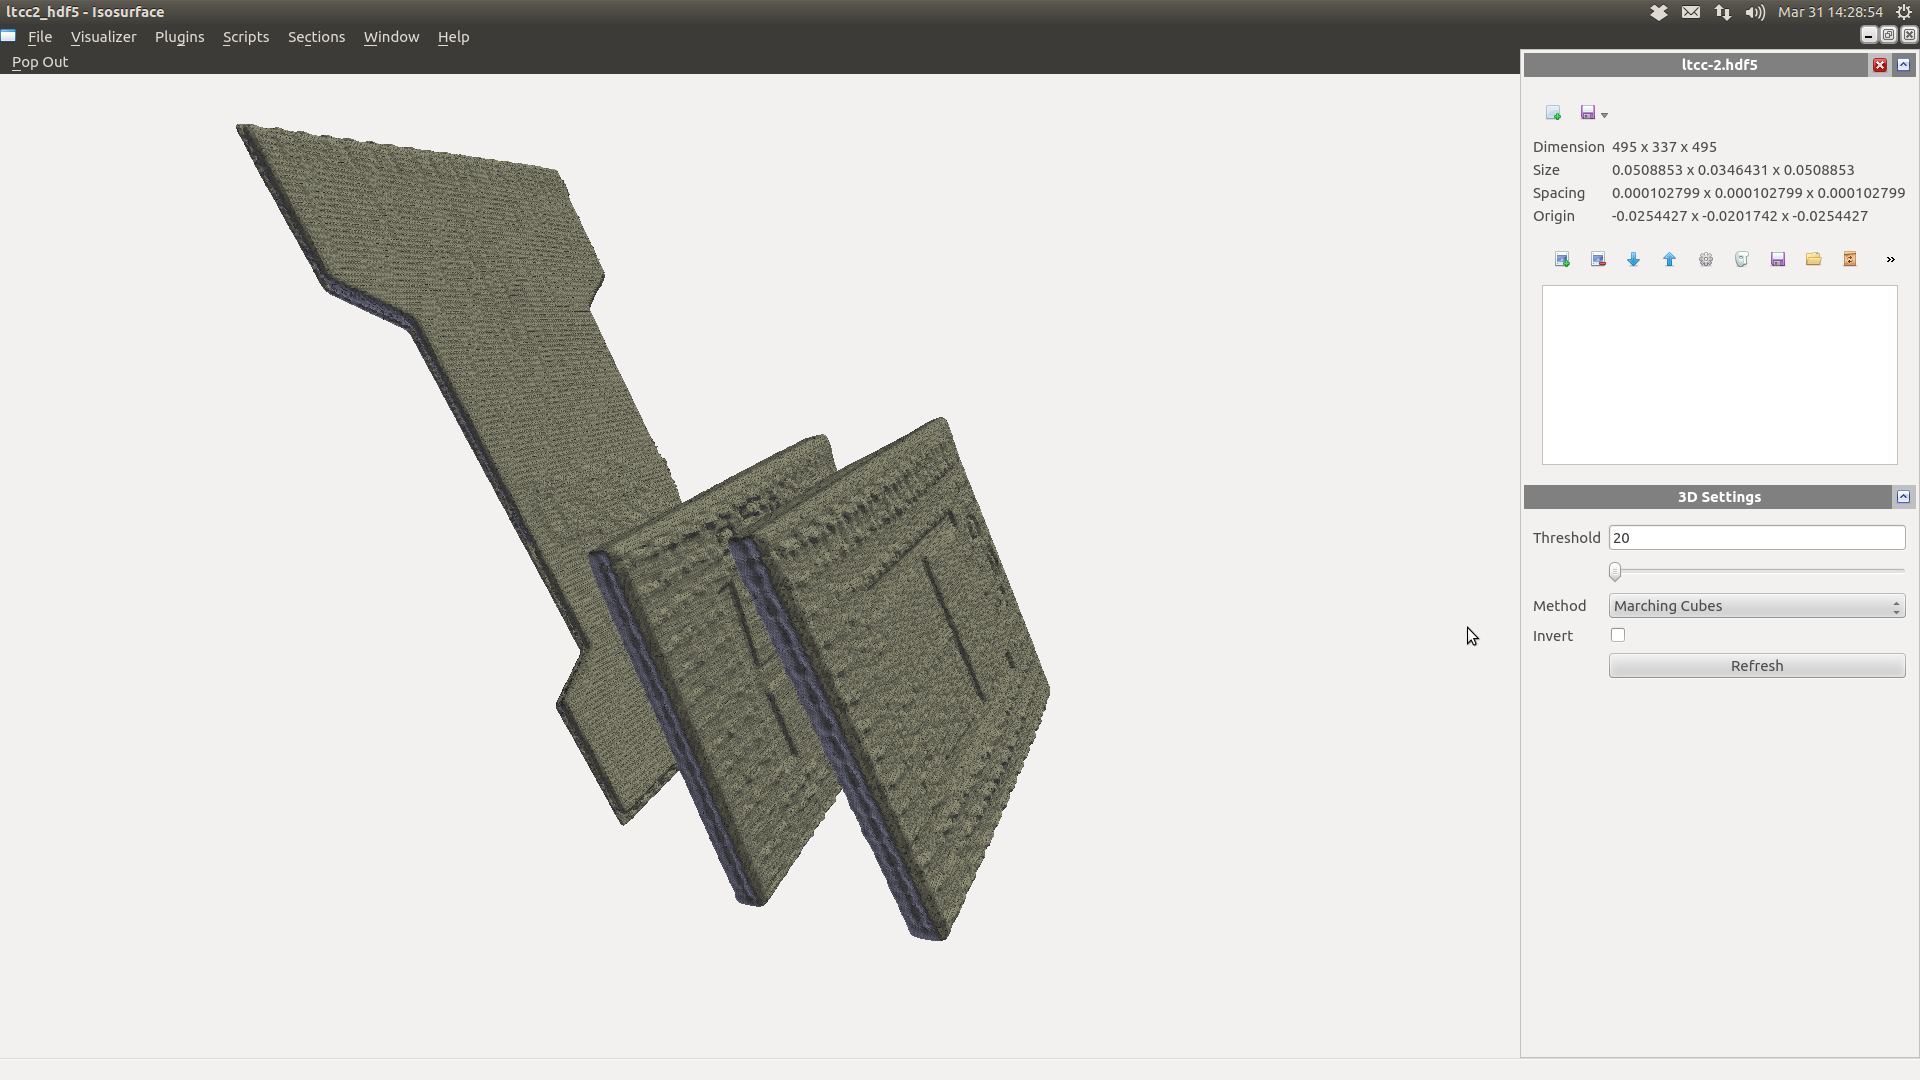
\includegraphics[width=1.0\textwidth]{img/isosurface.png}
\end{figure}

\newpage
\subsection{X-Ray}

The X-Ray visualizer allows seeing the data set as a whole piece. It accumulates
the voxels it finds while raycasting into the scene and thus shows the interior of
the data set.

It is useful to gather information about where specific structures are located in
the data set, if there are cavities in the data set or points with a high density.

\subsubsection{Settings}
The X-Ray visualizer can be set up via its side panel section.
The section has multiple options:
\begin{itemize}
	\item{\emph{Render Quality}\newline The number of samples used by the raycaster.
		Lower values are faster, higher values give more details.}
	\item{\emph{Minimum}\newline The minimum value considered as black/transparent.
		Can be used as an additional high-pass filter.}	
	\item{\emph{Maximum}\newline The maximum value considered as white/opaque.
			Can be used as a range adjustment.}
	\item{\emph{Result Scale}\newline Scales the result from the range options by
		a given amount. Can be used to tweak the image brightness.}
\end{itemize}
The settings the of visualizer are unit-less as the visualizer only provides a
visual representation that must be tweaked by eye.

For a computationally under-performing computer it is recommended to not use the
higher render quality settings as they draw a lot of computational power.

\subsubsection{Controls}
The data set can be rotated by dragging the mouse over the visualizer window while
holding down the left mouse button.
Scrolling the mouse wheel will zoom in or out the view.

\begin{figure}[h!]
	\caption{X-Ray}
	\centering
	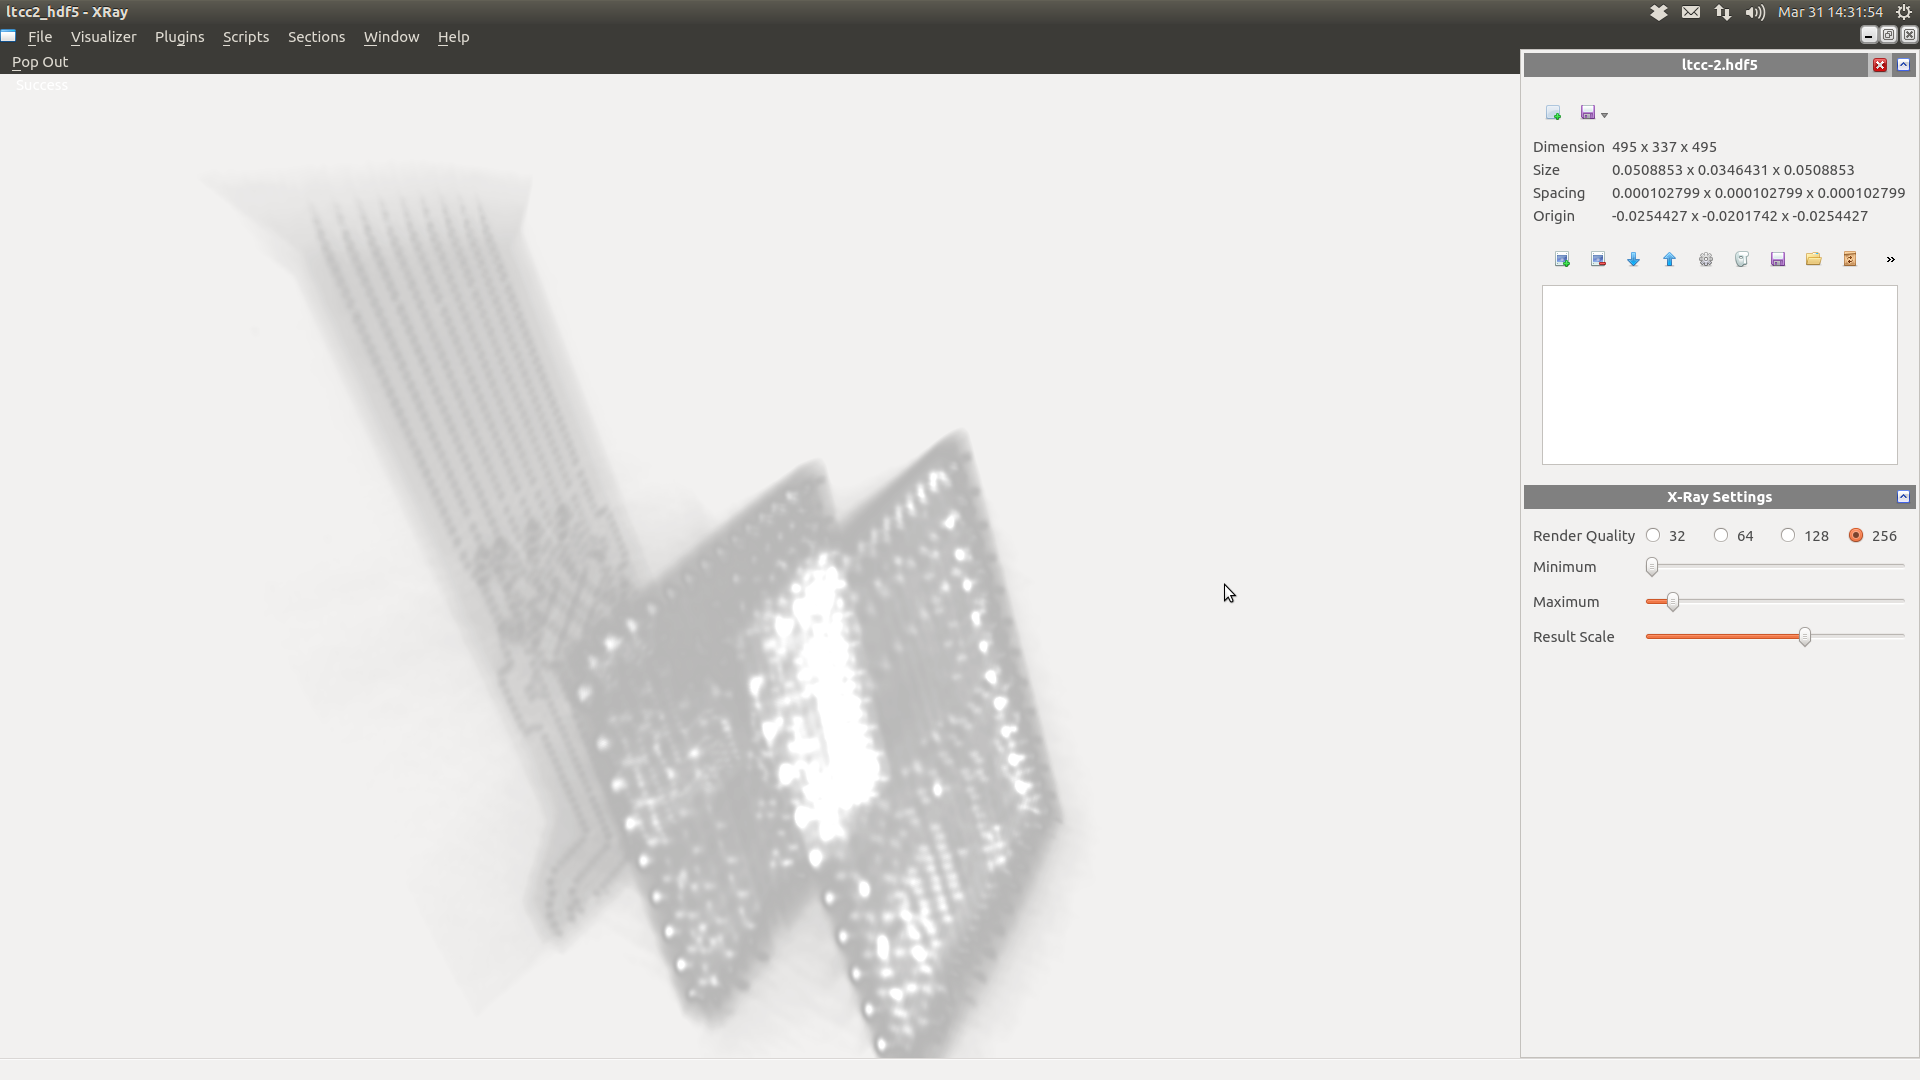
\includegraphics[width=1.0\textwidth]{img/x-ray.png}
\end{figure}